\chapter{Interface Screenshots \label{cha:appscreen}}

\section{Version Control Elements}

\begin{figure}[htb]
\centering
\setlength\fboxsep{0pt}
\setlength\fboxrule{0.5pt}
\fbox{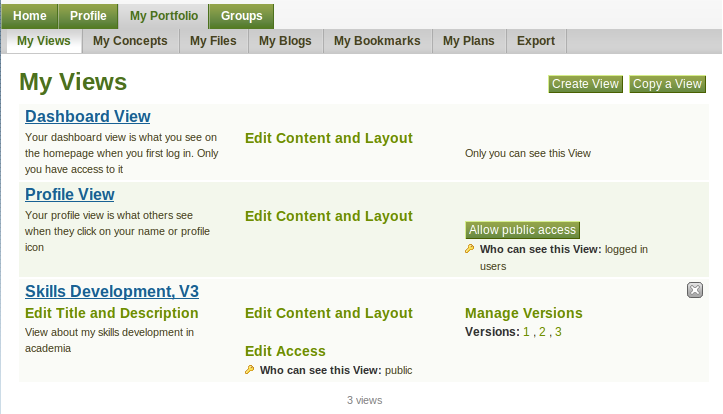
\includegraphics[width=0.95\textwidth]{AD-F1-V1}}
\caption[Views list]{Views list. The last view on the list has three versions}
\end{figure}

\begin{figure}[htb]
\centering
\setlength\fboxsep{0pt}
\setlength\fboxrule{0.5pt}
\fbox{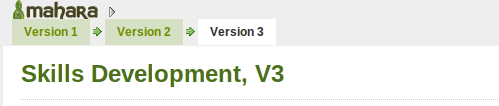
\includegraphics[width=0.95\textwidth]{AD-F1-V3}}
\caption{Navigation between versions}
\end{figure}

\begin{figure}[htb]
\centering
\setlength\fboxsep{0pt}
\setlength\fboxrule{0.5pt}
\fbox{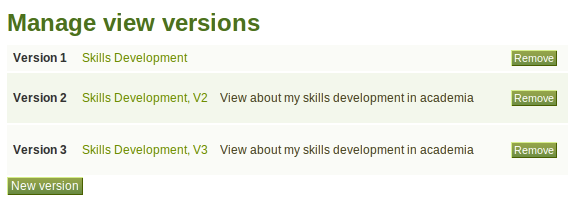
\includegraphics[width=0.95\textwidth]{AD-F1-V2}}
\caption{View versions management}
\end{figure}

%==================================================================
\section{Concept Mapping Module}
\begin{figure}[htb]
\centering
\setlength\fboxsep{0pt}
\setlength\fboxrule{0.5pt}
\fbox{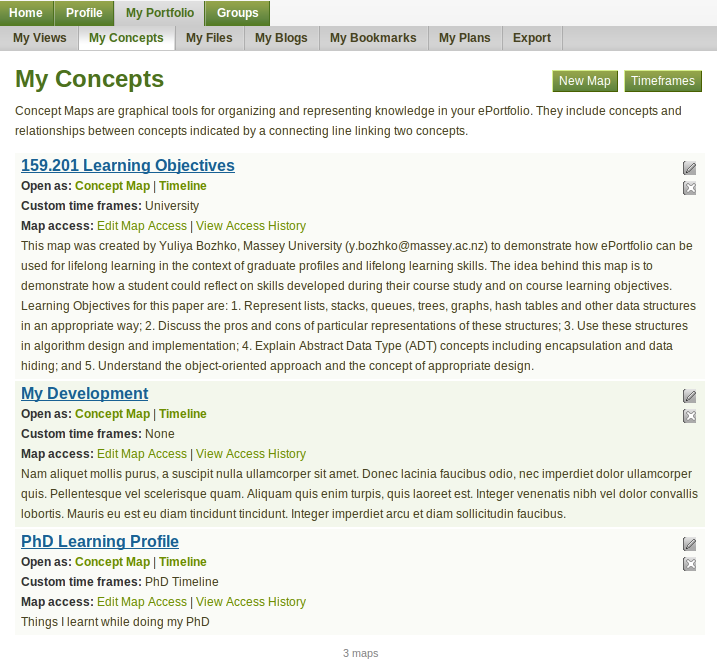
\includegraphics[width=0.95\textwidth]{AD-F2-Cmap1}}
\caption{Concept maps list}
\end{figure}
 
\begin{figure}[ht!]
\centering
\setlength\fboxsep{0pt}
\setlength\fboxrule{0.5pt}
\fbox{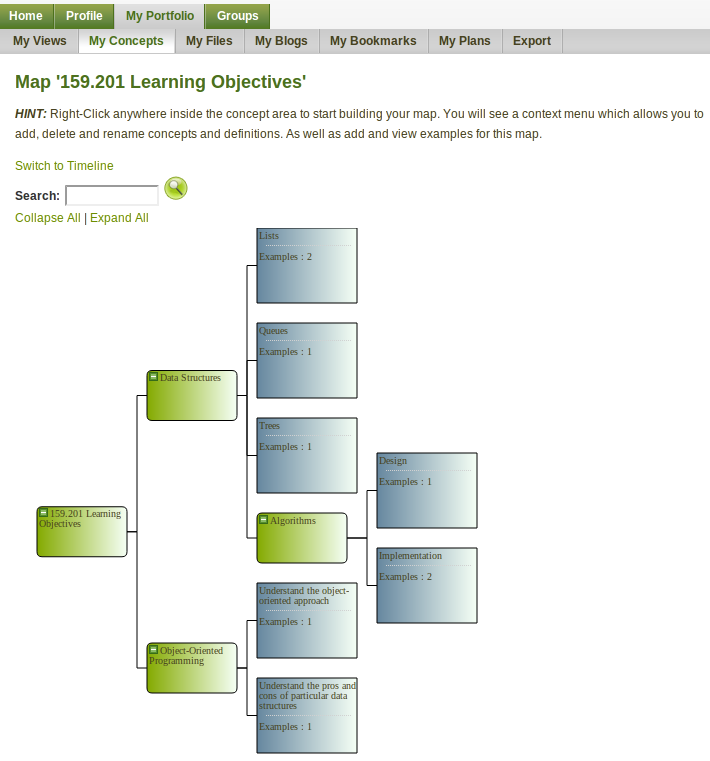
\includegraphics[width=0.95\textwidth]{AD-F2-Cmap2}}
\caption{Concepts layout in the form of map}
\end{figure}

\begin{figure}[ht!]
\centering
\setlength\fboxsep{0pt}
\setlength\fboxrule{0.5pt}
\fbox{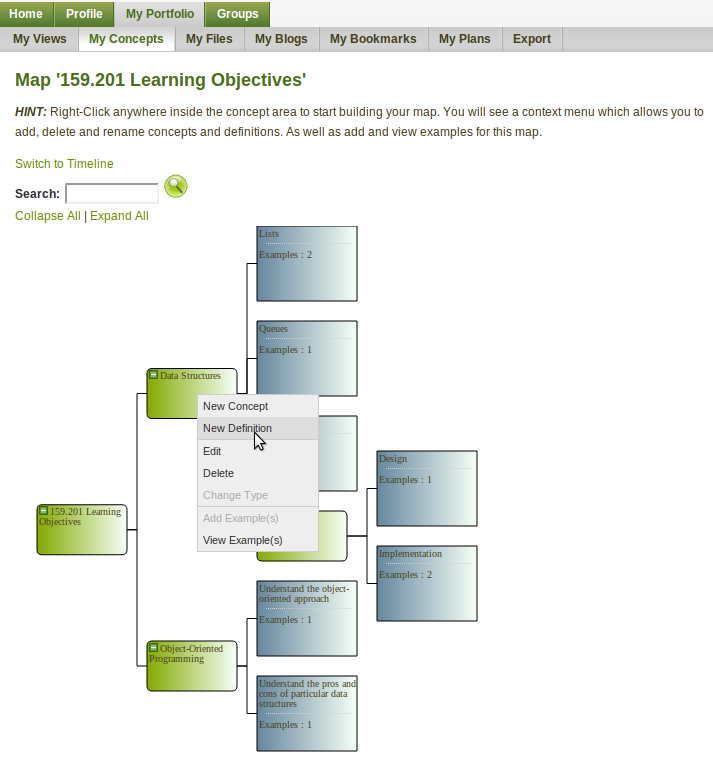
\includegraphics[width=0.95\textwidth]{AD-F2-Cmap3}}
\caption{Adding new items through the context menu}
\end{figure}

\begin{figure}[ht!]
\centering
\setlength\fboxsep{0pt}
\setlength\fboxrule{0.5pt}
\fbox{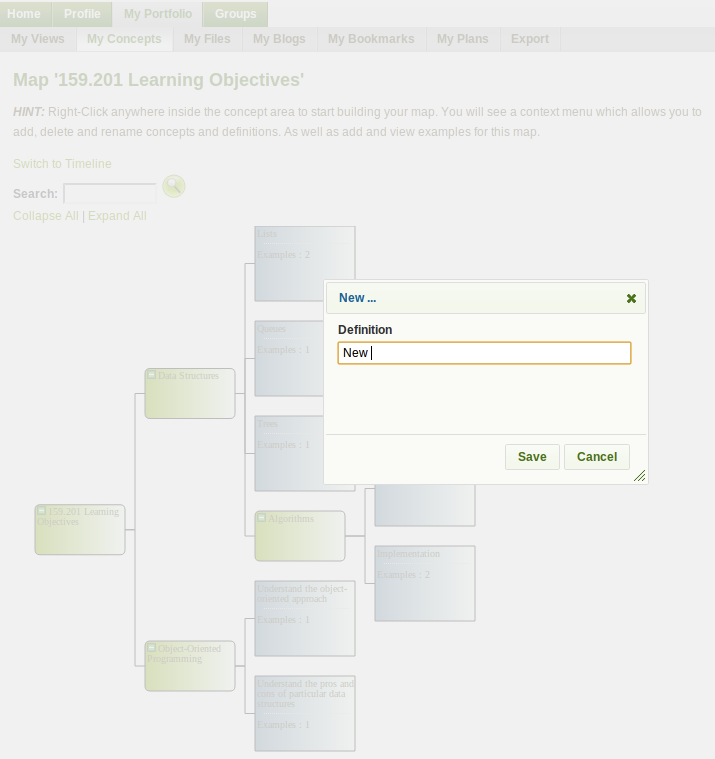
\includegraphics[width=0.95\textwidth]{AD-F2-Cmap4}}
\caption{Adding new definition to the map}
\end{figure}

\begin{figure}[ht!]
\centering
\setlength\fboxsep{0pt}
\setlength\fboxrule{0.5pt}
\fbox{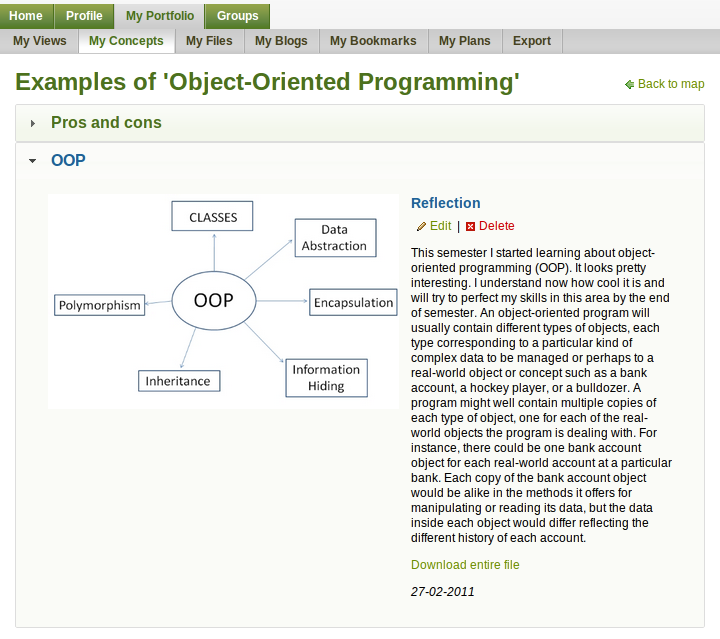
\includegraphics[width=0.95\textwidth]{AD-F2-Cmap5}}
\caption{A list of examples attached to the map}
\end{figure}

\FloatBarrier
%==================================================================

\section{Artifact Fragments Extraction}
 
\begin{figure}[ht!]
\centering
\setlength\fboxsep{0pt}
\setlength\fboxrule{0.5pt}
\fbox{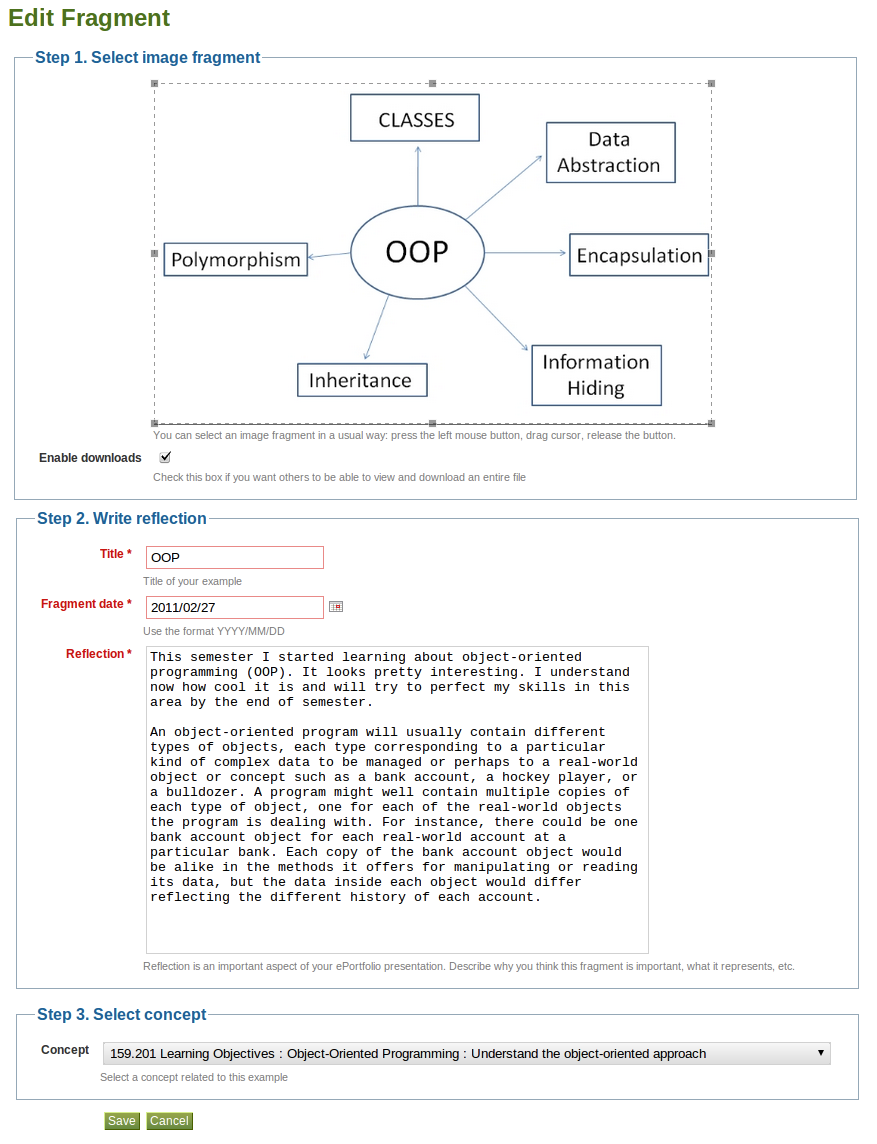
\includegraphics[width=0.95\textwidth]{AD-F3-Fragment}}
\caption{Artifact fragment layout}
\end{figure}

\begin{figure}[htb]
\centering
\setlength\fboxsep{0pt}
\setlength\fboxrule{0.5pt}
\fbox{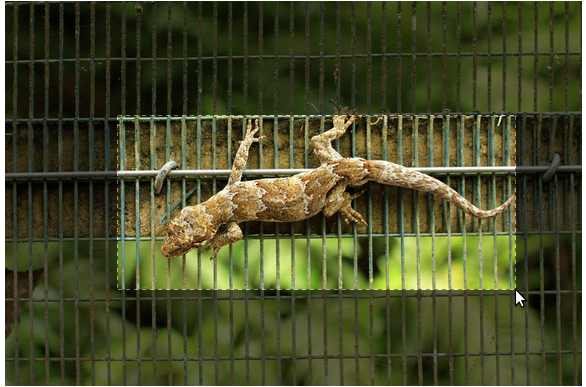
\includegraphics[width=0.95\textwidth]{AD-F3-Image}}
\caption{Taking image file fragment}
\end{figure}

\begin{figure}[htb]
\centering
\setlength\fboxsep{0pt}
\setlength\fboxrule{0.5pt}
\fbox{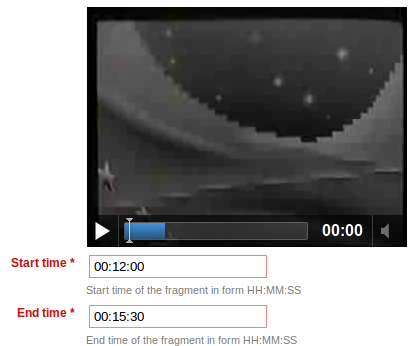
\includegraphics[width=0.90\textwidth]{AD-F3-Video}}
\caption{Taking video file fragment}
\end{figure}

\begin{figure}[htb]
\centering
\setlength\fboxsep{0pt}
\setlength\fboxrule{0.5pt}
\fbox{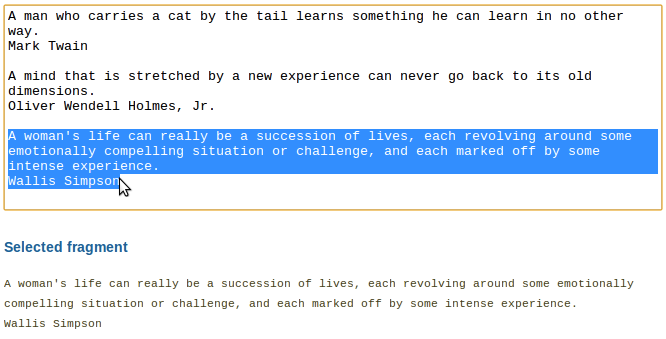
\includegraphics[width=0.95\textwidth]{AD-F3-Text}}
\caption{Taking text file fragment}
\end{figure}

\begin{figure}[htb]
\centering
\setlength\fboxsep{0pt}
\setlength\fboxrule{0.5pt}
\fbox{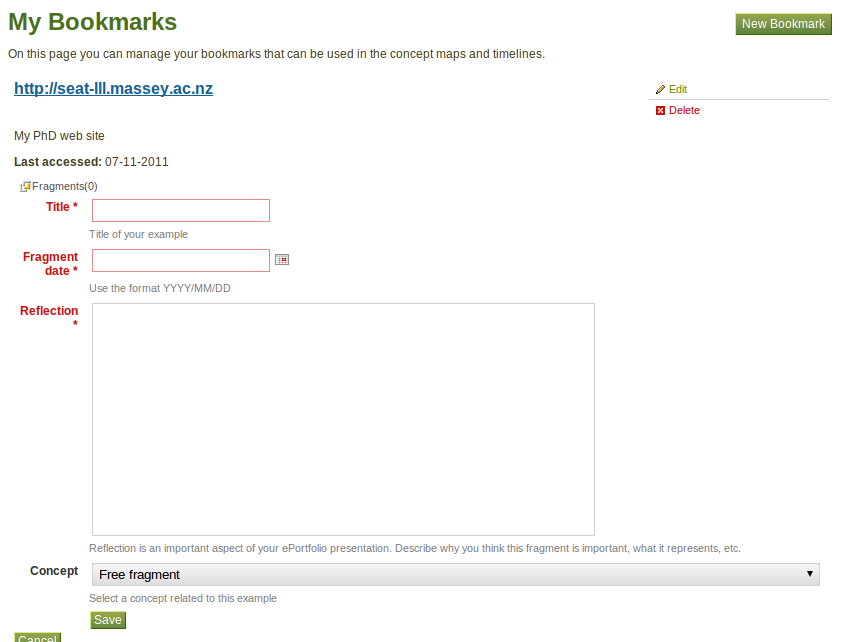
\includegraphics[width=0.95\textwidth]{AD-F3-Bookmark}}
\caption{Working with bookmarks}
\end{figure}

\FloatBarrier
%==================================================================

\section{Learning Progress Tracking}

\begin{figure}[ht!]
\centering
\setlength\fboxsep{0pt}
\setlength\fboxrule{0.5pt}
\fbox{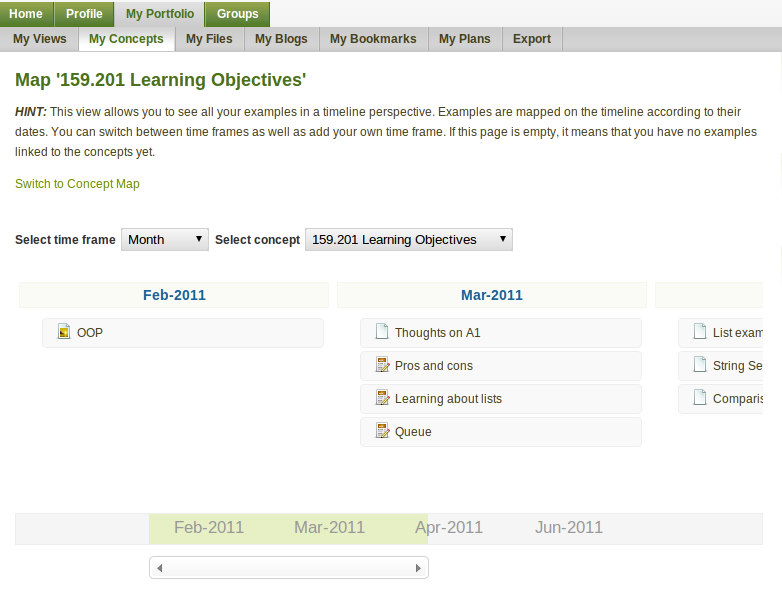
\includegraphics[width=0.95\textwidth]{AD-F4-Timeline1}}
\caption{Timeline layout of a map}
\end{figure}

\begin{figure}[ht!]
\centering
\setlength\fboxsep{0pt}
\setlength\fboxrule{0.5pt}
\fbox{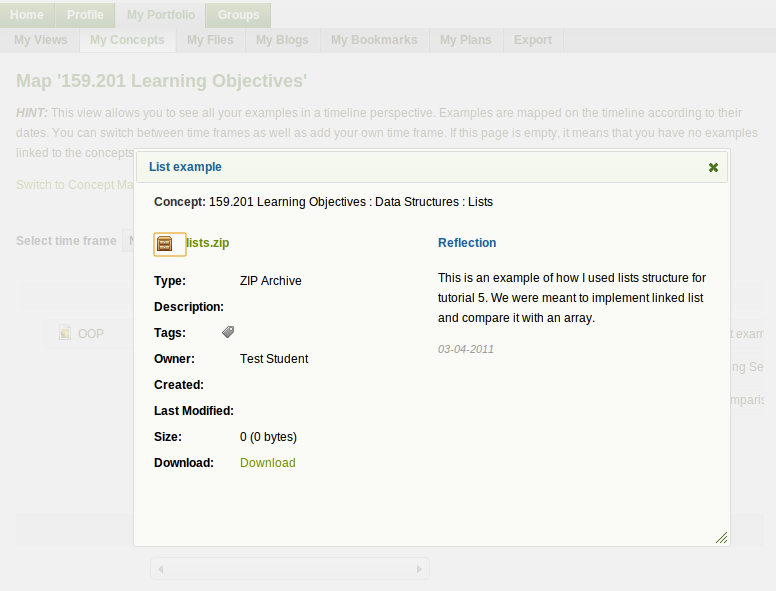
\includegraphics[width=0.95\textwidth]{AD-F4-Timeline2}}
\caption{An example window from a timeline page}
\end{figure}

\begin{figure}[ht!]
\centering
\setlength\fboxsep{0pt}
\setlength\fboxrule{0.5pt}
\fbox{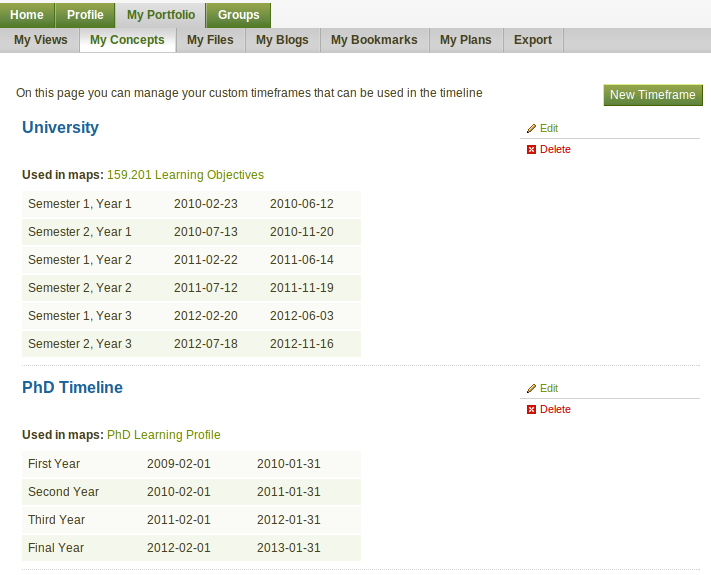
\includegraphics[width=0.95\textwidth]{AD-F4-Timeline3}}
\caption{Custom timeframes set-up page}
\end{figure}

\begin{figure}[htb]
\centering
\setlength\fboxsep{0pt}
\setlength\fboxrule{0.5pt}
\fbox{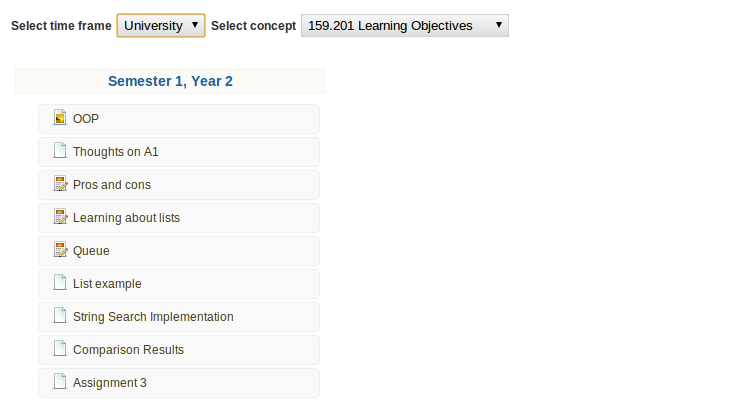
\includegraphics[width=0.95\textwidth]{AD-F4-Timeline4}}
\caption{Timeline filtered according to the custom timeframes}
\end{figure}

\FloatBarrier
%==================================================================

\section{Shared Resources Management}

\begin{figure}[ht!]
\centering
\setlength\fboxsep{0pt}
\setlength\fboxrule{0.5pt}
\fbox{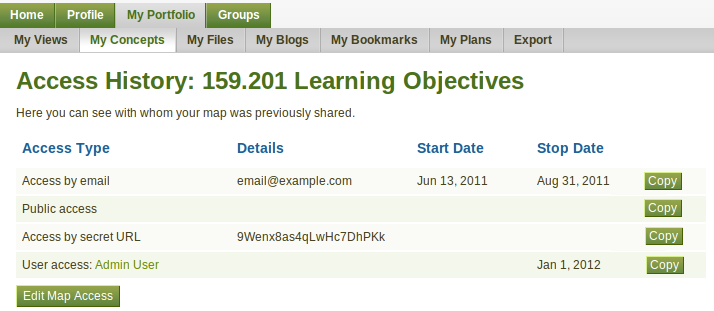
\includegraphics[width=0.95\textwidth]{AD-F5-History}}
\caption{History access log for a view}
\end{figure}